\documentclass{article}
\usepackage{adjustbox}
\usepackage{float}
\usepackage{textcomp}
\usepackage{graphicx}
\graphicspath{{images/}}
\usepackage{booktabs}
\usepackage{color}
\usepackage{verbatim}
\usepackage{listings}
\usepackage{underscore}
\setcounter{secnumdepth}{5}
\usepackage[bookmarks=true]{hyperref}
\author{Roberto Clapis (841859), Erica Stella (854443)} 
\date{\today}
\title{Politecnico di Milano
	\\A.A. 2015\@-\@2016
	\\Software Engineering 2: ``myTaxiService''
	\\\textbf{I}ntegration \textbf{T}est \textbf{P}lan \textbf{D}ocument}
\hypersetup{pdftitle={Integration Test Plan Document},    % title
	pdfauthor={Roberto Clapis, Erica Stella},                     % author
	pdfsubject={Integration Test Plan Document},                        % subject of the document
	pdfkeywords={TeX, LaTeX, taxi, ITPD, SoftwareEngineering2}, % list of keywords
	colorlinks=true,       % false: boxed links; true: colored links
	linkcolor=black,       % color of internal links
	citecolor=blue,       % color of links to bibliography
	filecolor=black,        % color of file links
	urlcolor=purple,        % color of external links
}
\begin{document}
\maketitle
\begin{center}
	
\includegraphics{polimi-logo}
\end{center}
\clearpage
\tableofcontents
\clearpage
\section{Introduction}
\subsection{Revision History}
%Record all revisions to the document
\subsection{Purpose and Scope}
%State the purpose and scope of the document
This document describes the Integration Test Plan for the myTaxiService application. It provides a plan referring to how the various components 
described in the Design Document will be integrated for testing. 
\subsection{List of Definitions and Abbreviations}
\begin{itemize}
	\item \textit{UI:} User Interface.
	\item \textit{Database's stubs:} Active Requests and Reservations' stub 
	and Accounts' stub.
	\item \textit{UIs' stubs:} ClientUI's stub and DriverUI's stub.
\end{itemize}
\subsection{List of Reference Documents}
%List all reference documents, for instance: the project description, the RASD, the Design document, the documentation of any tool you plan to use for testing
\begin{itemize}
	\item The document with myTaxiService's description
	\item myTaxiService's RASD
	\item myTaxiService's Design Document
\end{itemize}
\section{Integration Strategy}
\subsection{Entry Criteria}
%Specify the criteria that must be met before integration testing of specific elements may begin (e.g., functions must have been unit tested).
Before the integration testing, each single module must have been tested to verify the correct functioning of its methods according to its specifications.
\subsection{Elements to be Integrated}
%Identify the components to be integrated, refer to your design document to identify such components in a way that is consistent with your design 
According to the Design Document, the components to be integrated are:
\begin{itemize}
	\item Database: 
	\begin{itemize}
		\item Accounts
		\item Active Reservations and Requests
	\end{itemize}
	\item Web Server: 
	\begin{itemize}
		\item DBConnector
		\item APIBackend
		\item WebpageCreator
		\item NotificationModule
		\item HttpHandler
	\end{itemize}
	\item UI:\@
	\begin{itemize}
		\item ClientUI
		\item DriverUI
		\item AdminUI
	\end{itemize}
\end{itemize}
\subsection{Integration Testing Strategy}
%Describe the integration testing approach (top-down, bottom-up, functional groupings, etc.) and the rationale for the choosing that approach
The decided testing approach is sandwich. This has been chosen in order to 
integrate first the components of the WebServer, and then integrate the WebServer with the Database and the UI. %TODO finire di aggiungere la motivazione
%TODO Aspetta, a sandwich non è l'esatto opposto?

\subsection{Sequence of Component/Function Integration}
%NOTE: the structure of this section may vary depending on the integration strategy you select in Section 2.3. Use the structure proposed below as a non mandatory guide
\subsubsection{Software Integration Sequence}
%For each subsystem: identify the sequence in which the software components will be integrated within the subsystem. Relate this sequence to any product features/functions that are being built up
In the following graphs the arrows go 
from the called module to the caller module
and are marked with identifiers that define
the order of integration.
\paragraph{Web Server}
The following images describe how the Web Server's 
components will be integrated for testing.
\begin{figure}[H]
		\makebox[\textwidth][c]{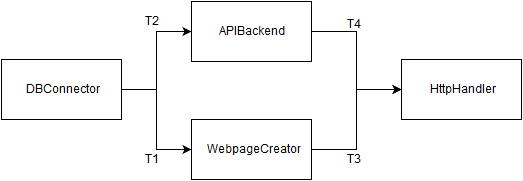
\includegraphics[width=1.0\textwidth]{WebServer1}}%
\end{figure}
\begin{figure}[H]
	\makebox[\textwidth][c]{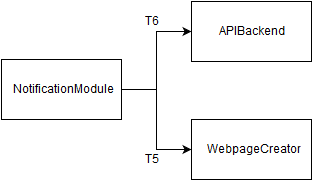
\includegraphics[width=0.7\textwidth]{WebServer2}}%
\end{figure}
\subsubsection{Subsystem Integration Sequence}
%Identify the order in which subsystems will be integrated. If you have a single subsystem, 2.4.1 and 2.4.2 are to be merged in a single section. You can refer to Section 2.2 of the test plan example [1] as an example of what we expect
The following graphs describe how the three 
main components of myTaxiService application, 
the Database, the Web Server and 
the UIs, will be integrated.
\begin{figure}[H]
	\makebox[\textwidth][c]{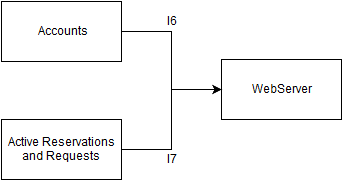
\includegraphics[width=0.7\textwidth]{DBWS}}%
\end{figure}
\begin{figure}[H]
	\makebox[\textwidth][c]{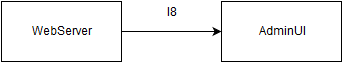
\includegraphics[width=0.65\textwidth]{WSUI3}}%
\end{figure}
\begin{figure}[H]
	\makebox[\textwidth][c]{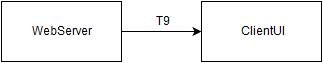
\includegraphics[width=0.65\textwidth]{WSUI1}}%
\end{figure}
\begin{figure}[H]
	\makebox[\textwidth][c]{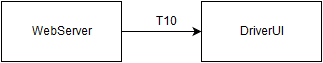
\includegraphics[width=0.65\textwidth]{WSUI2}}%
\end{figure}
\section{Individual Steps and Test Description}
%For each step of the integration process identified above, describe the type of tests that will be used to verify that the elements integrated in this step perform as expected. Describe in general the expected results of the test set. You may refer to Chapter 3 and Chapter 4 of the test plan example [1] as an example of what we expect. (NOTE: this is not a detailed description of test protocols. Think of this as the test design phase. Specific protocols will be written to fulfill the goals of the tests identified in this section.)
\subsection{Test case specifications}
\subsubsection{I1}
\begin{adjustbox}{width=1.2\textwidth}	
	\begin{tabular}{*{2}{p{0.6\textwidth}}}
		\toprule
		\textbf{Test Case identifier} & I1T1\\
		\textbf{Test Items} & DBConnector $\rightarrow$ WebpageCreator\\
		\textbf{Input Specification} & Perform valid and invalid requests on the WebPage Creator\\
		\textbf{Output Specification} & All and only the queries that should be allowed are executed and the correct DBConnector's methods are called\\
		\textbf{Environmental Needs} & Database's stub, WebpageCreator driver\\
		\bottomrule
	\end{tabular}
\end{adjustbox}
\subsubsection{I2}
\begin{adjustbox}{width=1.2\textwidth}	
	\begin{tabular}{*{2}{p{0.6\textwidth}}}
		\toprule
		\textbf{Test Case identifier} & I2T1\\
		\textbf{Test Items} & DBConnector $\rightarrow$ APIBackend\\
		\textbf{Input Specification} & Perform valid and invalid requests on the APIBackend\\
		\textbf{Output Specification} & All and only the queries that should be allowed are executed and the correct DBConnector's methods are called\\
		\textbf{Environmental Needs} & Database's stub, APIBackend driver\\
		\bottomrule
	\end{tabular}
\end{adjustbox}
\subsubsection{I3}
\begin{adjustbox}{width=1.2\textwidth}	
	\begin{tabular}{*{2}{p{0.6\textwidth}}}
		\toprule
		\textbf{Test Case identifier} & I3T1\\
		\textbf{Test Items} & WebpageCreator $\rightarrow$ HttpHandler\\
		\textbf{Input Specification} & Perform valid and invalid requests on the HttpHandler\\
		\textbf{Output Specification} & Verify if only the requests intended for 
		the WebpageCreator are forwarded to it and the correct WebpageCreator methods are called\\
		\textbf{Environmental Needs} & Database's stub, HttpHandler driver, I1,I2 successful\\
		\bottomrule
	\end{tabular}
\end{adjustbox}
\begin{adjustbox}{width=1.2\textwidth}	
	\begin{tabular}{*{2}{p{0.6\textwidth}}}
		\toprule
		\textbf{Test Case identifier} & I3T2\\
		\textbf{Test Items} & APIBackend $\rightarrow$ HttpHandler\\
		\textbf{Input Specification} & Perform valid and invalid requests on the HttpHandler\\
		\textbf{Output Specification} & Verify if only the requests intended for
		the APIBackend are forwarded to it and the correct APIBacken methods are called\\
		\textbf{Environmental Needs} & Active Requests and Reservations' stub, Accounts' stub, HttpHandler driver, I1,I2 successful\\
		\bottomrule
	\end{tabular}
\end{adjustbox}
\subsubsection{I4}
\begin{adjustbox}{width=1.2\textwidth}	
	\begin{tabular}{*{2}{p{0.6\textwidth}}}
		\toprule
		\textbf{Test Case identifier} & I4T1\\
		\textbf{Test Items} & NotificationModule $\rightarrow$ WebpageCreator\\
		\textbf{Input Specification} & All the possible types of input that require sending notifications to a client \\ 
		\textbf{Output Specification} & Check if the correct methods of the NotificationModule have been called\\
		\textbf{Environmental Needs} & UIs' stub, WebpageCreator driver\\
		\bottomrule
	\end{tabular}
\end{adjustbox}
\subsubsection{I5}
\begin{adjustbox}{width=1.2\textwidth}	
	\begin{tabular}{*{2}{p{0.6\textwidth}}}
		\toprule
		\textbf{Test Case identifier} & I5T1\\
		\textbf{Test Items} & NotificationModule $\rightarrow$ APIBackend\\
		\textbf{Input Specification} & All the possible types of input that require sending notifications to a client \\ 
		\textbf{Output Specification} & Check if the correct methods of the NotificationModule have been called\\
		\textbf{Environmental Needs} & UIs' stub, APIBackend driver\\
		\bottomrule
	\end{tabular}
\end{adjustbox}
\subsubsection{I6}
\begin{adjustbox}{width=1.2\textwidth}	
	\begin{tabular}{*{2}{p{0.6\textwidth}}}
		\toprule
		\textbf{Test Case identifier} & I6T1\\
		\textbf{Test Items} & Accounts $\rightarrow$ WebServer\\
		\textbf{Input Specification} & Queries to manipulate (creation modification and deletion) of accounts\\
		\textbf{Output Specification} & The correct Accounts' method have been called\\
		\textbf{Environmental Needs} & WebServer driver, Active Reservations and Requests' stub, I1-15 successful\\
		\bottomrule
	\end{tabular}
\end{adjustbox}
\subsubsection{I7}
\begin{adjustbox}{width=1.2\textwidth}	
	\begin{tabular}{*{2}{p{0.6\textwidth}}}
		\toprule
		\textbf{Test Case identifier} & I7T1\\
		\textbf{Test Items} & Active Reservations and Requests $\rightarrow$ WebServer\\
		\textbf{Input Specification} & Queries to place/accept/delete reservations and requests, in every possible order of execution\\ 
		\textbf{Output Specification} & The correct Active Reservations and Requests' methods have been called\\
		\textbf{Environmental Needs} & WebServer driver, I1-I6 successful\\
		\bottomrule
	\end{tabular}
\end{adjustbox}
\subsubsection{I8}
\begin{adjustbox}{width=1.2\textwidth}	
	\begin{tabular}{*{2}{p{0.6\textwidth}}}
		\toprule
		\textbf{Test Case identifier} & I8T1\\
		\textbf{Test Items} & WebServer $\rightarrow$ AdminUI\\
		\textbf{Input Specification} & Every possible input from the UI\\ 
		\textbf{Output Specification} & The correct WebServer's methods have been called\\
		\textbf{Environmental Needs} & I1-I7 successful\\
		\bottomrule
	\end{tabular}
\end{adjustbox}
\subsubsection{I9}
\begin{adjustbox}{width=1.2\textwidth}	
	\begin{tabular}{*{2}{p{0.6\textwidth}}}
		\toprule
		\textbf{Test Case identifier} & I9T1\\
		\textbf{Test Items} & WebServer $\rightarrow$ ClientUI\\
		\textbf{Input Specification} & Every possible input from the UI\\ 
		\textbf{Output Specification} & The correct WebServer's methods have been called\\
		\textbf{Environmental Needs} & I1-I7 successful\\
		\bottomrule
	\end{tabular}
\end{adjustbox}
\subsubsection{I10}
\begin{adjustbox}{width=1.2\textwidth}	
	\begin{tabular}{*{2}{p{0.6\textwidth}}}
		\toprule
		\textbf{Test Case identifier} & I10T1\\
		\textbf{Test Items} & WebServer $\rightarrow$ AdminUI\\
		\textbf{Input Specification} & Every possible input from the UI\\ 
		\textbf{Output Specification} & The correct WebServer's methods have been called\\
		\textbf{Environmental Needs} & I1-I7 successful\\
		\bottomrule
	\end{tabular}
\end{adjustbox}
\subsection{Integration Test Procedures}
\subsubsection{TP1}
\begin{adjustbox}{width=1.2\textwidth}	
	\begin{tabular}{*{2}{p{0.6\textwidth}}}
		\midrule
		\textbf{Test Procedure Identifier} & TP1\\
		\textbf{Purpose} & This test procedure verifies whether the WebServer's components work properly together with all kinds of inputs\\ 
		\textbf{Procedure Steps} & Execute I1-I5\\
		\bottomrule
	\end{tabular}
\end{adjustbox}
\subsubsection{TP2}
\begin{adjustbox}{width=1.2\textwidth}	
	\begin{tabular}{*{2}{p{0.6\textwidth}}}
		\midrule
		\textbf{Test Procedure Identifier} & TP2\\
		\textbf{Purpose} & This test procedure verifies whether the Database can handle all types of inputs and modifications requested by the WebServer\\ 
		\textbf{Procedure Steps} & Execute I6-I7\\
		\bottomrule
	\end{tabular}
\end{adjustbox}
\subsubsection{TP3}
\begin{adjustbox}{width=1.2\textwidth}	
	\begin{tabular}{*{2}{p{0.6\textwidth}}}
		\midrule
		\textbf{Test Procedure Identifier} & TP3\\
		\textbf{Purpose} & This test procedure verifies whether the WebServer can handle all the inputs from the UIs and outputs the requested information\\ 
		\textbf{Procedure Steps} & Execute I8-I10\\
		\bottomrule
	\end{tabular}
\end{adjustbox}
\section{Tools and Test Equipment Required}
%Identify all tools and test equipment needed to accomplish the integration. Refer to the tools presented during the lectures. Explain why and how you're going to use them. Note that you may also use manual testing for some part. Consider manual testing as one of the possible tools you have available.
We base our tools' choice on the assumption that
the implementation of the myTaxiService application
has been made using Java as programming language.
As one of the most used and reliable testing frameworks
currently available, we decided to exploit the
functionalities of Mockito. In particular, it
has been used to create all the stubs and the drivers
named in Section 3.1.
\section{Program Stubs and Test Data Required}
%Based on the testing strategy and test design, identify any program stubs or special test data required for each integration step.
\subsection{Stubs}
The required stubs are:
\begin{itemize}
	\item Active Requests and Reservations' stub
	\item Accounts' stub
	\item ClientUI's stub
	\item DriverUI's stub
\end{itemize}
For the complete set of methods exposed by the 
interfaces of the modules listed above refer
to the Design Document's section 2.6.
\subsubsection{Database' stub}
This stubs should simulate a real database. They 
should provide responses for all the possible contents 
a database could have.
\subsubsection{UIs's stub}
These stubs are used only in the NotificationModule's test.
They have to mock the reception of messages from the WebServer.
\subsection{Drivers}
As stated in Section 3.1, all tests except for I8-I10 need 
a driver. They are used to provide the inputs that should cover
all the possible inputs the module could receive, where possible, 
and check the output for correctness.
\end{document}
